\documentclass[xetex,mathserif,serif]{beamer}
\usepackage{polyglossia}
\setdefaultlanguage[babelshorthands=true]{russian}
\usepackage{minted}

\useoutertheme{infolines}

\setmainfont{FreeSans}
\newfontfamily{\russianfonttt}{FreeSans}

\title{Проектирование ПО}
\author[Юрий Литвинов]{Юрий Литвинов \newline \textcolor{gray}{\small\texttt{yurii.litvinov@gmail.com}}}
\date{27.03.2017г}

\begin{document}
	
	\frame{\titlepage}
	
	\section{Введение}

	\begin{frame}
		\frametitle{Проектирование ПО}
		Проектирование --- деятельность, предшествующая разработке
		\vskip 1.5cm
		\begin{center}
			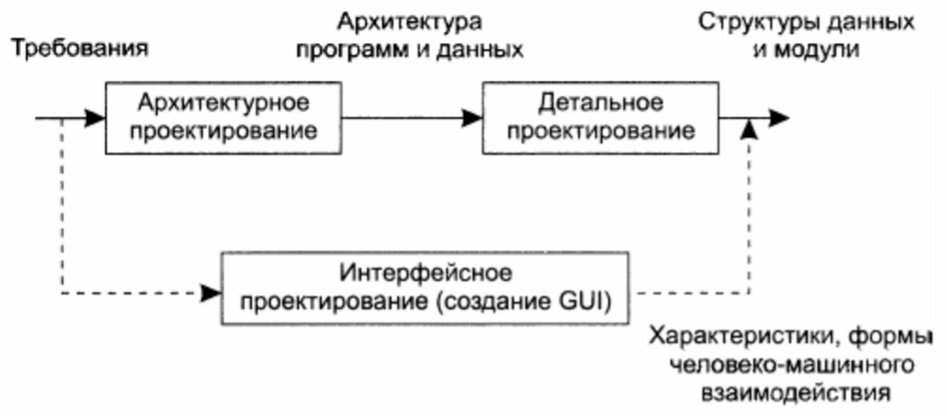
\includegraphics[width=0.7\textwidth]{softwareDesign.png}
		\end{center}
	\end{frame}

	\begin{frame}
		\frametitle{Проектирование ПО}
		\begin{itemize}
			\item Определение базового архитектурного стиля и структуры приложения
			\item Определение функционального поведения
			\item Осуществление декомпозиции на модули и планирование их взаимодействия
			\item Выбор стратегии и деталей реализации
			\begin{itemize}
				\item Используется ли кодогенерация?
				\item Используются ли сторонние фреймворки?
				\item Используются ли сторонние библиотеки?
				\item Какая часть функциональности будет реализовывать ``вручную''?
			\end{itemize}
			\item Вопросы распределённости/децентрализованности приложения
			\item Вопросы безопасности и прочие нефункциональные требования
			\item Вопросы локализации
			\item Вопросы размещения
			\item Вопросы обновления
			\item ...
		\end{itemize}
	\end{frame}

	\begin{frame}
		\frametitle{Инструменты проектирования}
		\begin{itemize}
			\item Моделирование
			\begin{itemize}
				\item Визуальное
				\item Вербальное
				\item Формальное
			\end{itemize}
			\item Прототипирование
			\item Архитектурное описание
			\begin{itemize}
				\item Неформальное
				\item Формальное
			\end{itemize}
		\end{itemize}
	\end{frame}

	\begin{frame}
		\frametitle{Моделирование}
		\begin{itemize}
			\item \textbf{Модель} --- упрощённое подобие объектов или явлений
			\begin{itemize}
				\item Позволяет изучать некоторые их свойства
			\end{itemize}
			\item Свойства моделей
			\begin{itemize}
				\item Сжатие информации
				\item Целенаправленность
				\item Субъективность
				\item Ограниченность
				\item Способность к расширению
			\end{itemize}
		\end{itemize}
	\end{frame}

	\begin{frame}
		\frametitle{Визуальные модели}
		\begin{columns}
			\begin{column}{0.5\textwidth}
				\begin{itemize}
					\item Различный состав моделей и степень детальности
					\item Метафора визуализации
					\item Точка зрения моделирования
					\item Назначение
					\begin{itemize}
						\item Одноразовые модели
						\item Документация
						\item Графические исходники
					\end{itemize}
				\end{itemize}
			\end{column}
			\begin{column}{0.5\textwidth}
				\begin{center}
					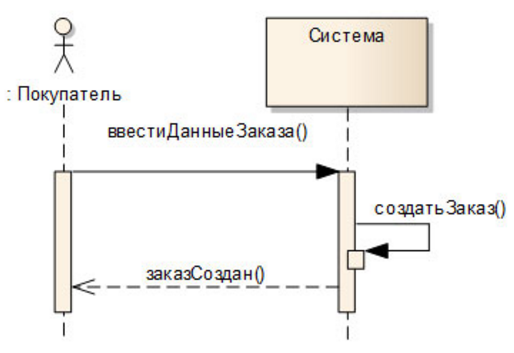
\includegraphics[width=0.9\textwidth]{modelExample.png}
				\end{center}
			\end{column}
		\end{columns}
	\end{frame}

	\section{UML, моделирование структуры}

	\begin{frame}
		\frametitle{Язык UML}
		\framesubtitle{Unified Modeling Language}
		\begin{center}
			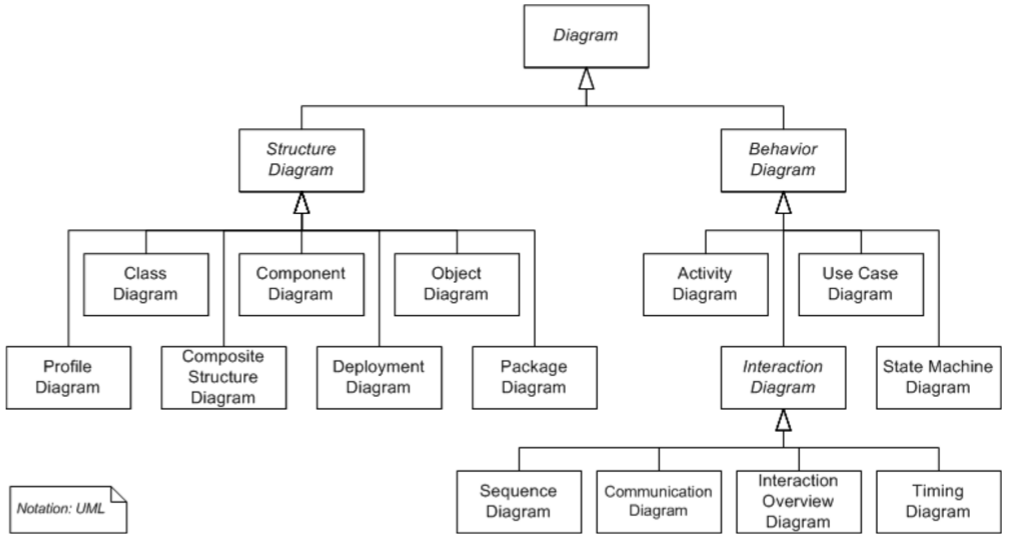
\includegraphics[width=\textwidth]{umlDiagrams.png}
		\end{center}
	\end{frame}

	\begin{frame}
		\frametitle{Представления системы}
		\begin{center}
			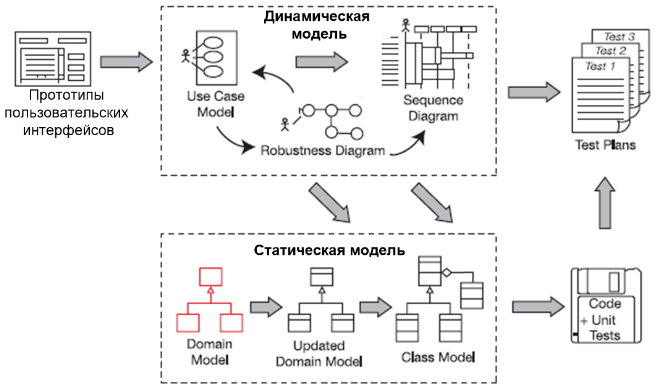
\includegraphics[width=0.8\textwidth]{modelTypes.png}
		\end{center}
	\end{frame}

	\begin{frame}
		\frametitle{Моделирование структуры}
		\begin{itemize}
			\item Отношения ``часть-целое''
			\item Статические свойства
			\item Не рассматриваем
			\begin{itemize}
				\item ``Причина-следствие''
				\item ``Раньше-позже''
			\end{itemize}
			\item Основные сущности --- пакеты, классы и отношения между ними
		\end{itemize}
	\end{frame}

	\begin{frame}
		\frametitle{Что моделируем}
		\begin{itemize}
			\item Структура связей между объектами во время выполнения программы
			\item Структура хранения данных
			\item Структура программного кода
			\item Структура компонентов в приложении
			\item Структура артефактов в проекте
			\item Структура используемых вычислительных ресурсов
		\end{itemize}
	\end{frame}

	\begin{frame}
		\frametitle{Диаграммы классов UML}
		\begin{center}
			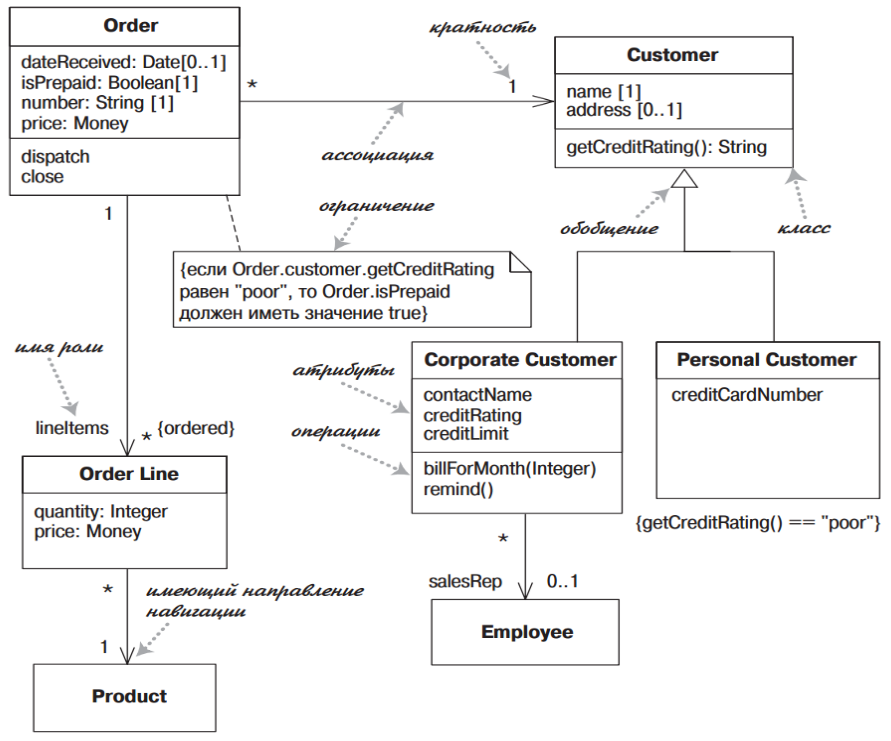
\includegraphics[width=0.7\textwidth]{umlClassDiagram.png}
		\end{center}
	\end{frame}

	\begin{frame}
		\frametitle{Свойства}
		\begin{columns}
			\begin{column}{0.3\textwidth}
				\begin{center}
					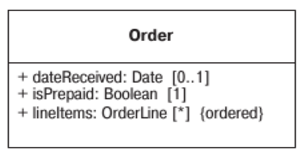
\includegraphics[width=0.8\textwidth]{attributes.png}

					Атрибуты
				\end{center}
			\end{column}
			\begin{column}{0.7\textwidth}
				\begin{center}
					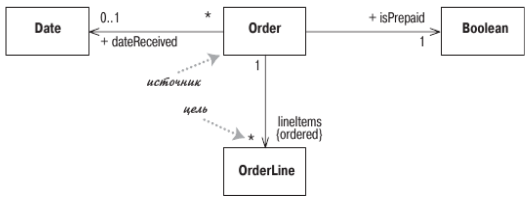
\includegraphics[width=0.7\textwidth]{associations.png}

					Ассоциации
				\end{center}
			\end{column}
		\end{columns}
		\bigskip
		Синтаксис:
		\begin{itemize}
			\item видимость имя: тип кратность = значение по умолчанию \{строка свойств\}
			\item Видимость: + (public), - (private), \# (protected), \char`~ (package)
			\item Кратность: 1 (ровно 1 объект), 0..1 (ни одного или один),\newline * (сколько угодно), 1..*, 2..*
		\end{itemize}
	\end{frame}

	\begin{frame}
		\frametitle{Агрегация и композиция}
		Агрегация – объект ``знает'' о другом (не управляет его временем жизни, имеет на него ссылку или указатель)
		\begin{center}
			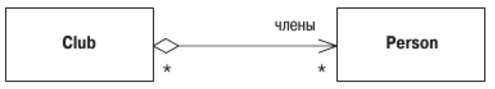
\includegraphics[width=0.5\textwidth]{aggregations.png}
		\end{center}
		Композиция --- объект владеет другим объектом (управляет его временем жизни, хранит его по значению или по указателю, делая delete)
		\begin{center}
			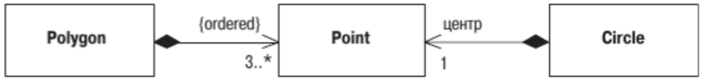
\includegraphics[width=0.7\textwidth]{compositions.png}
		\end{center}
		Уточнение обычной ассоциации, используется только если очень надо
	\end{frame}

	\begin{frame}
		\frametitle{Прочее}
		\begin{columns}
			\begin{column}{0.5\textwidth}
				\begin{center}
					Интерфейсы

					\bigskip
					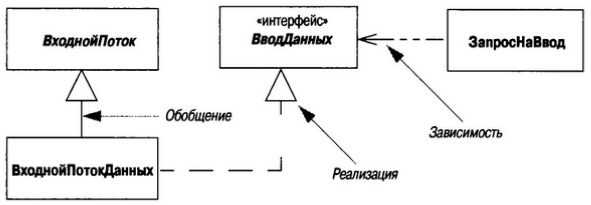
\includegraphics[width=0.9\textwidth]{interfaces1.png}

					\bigskip
					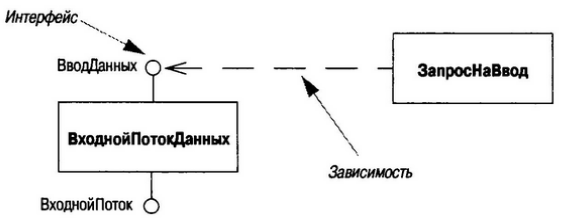
\includegraphics[width=0.9\textwidth]{interfaces2.png}
				\end{center}
			\end{column}
			\begin{column}{0.5\textwidth}
				\begin{center}
					Зависимости

					\bigskip
					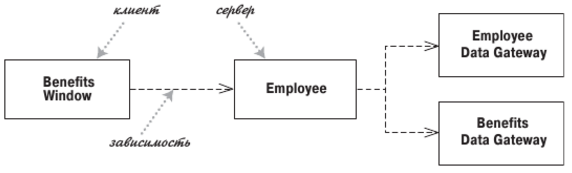
\includegraphics[width=0.9\textwidth]{dependencies.png}
					\bigskip

					Шаблоны

					\bigskip
					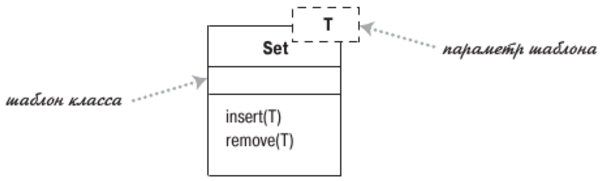
\includegraphics[width=0.9\textwidth]{templates.png}
				\end{center}
			\end{column}
		\end{columns}
	\end{frame}

	\begin{frame}
		\frametitle{Диаграммы объектов}
				\begin{columns}
			\begin{column}{0.5\textwidth}
				\begin{itemize}
					\item snapshot структуры классов во время выполнения
					\item Используются обычно чтобы пояснить диаграмму классов
					\item Полезны на этапе анализа предметной области, ещё до диаграмм классов
				\end{itemize}
			\end{column}
			\begin{column}{0.5\textwidth}
				\begin{center}
					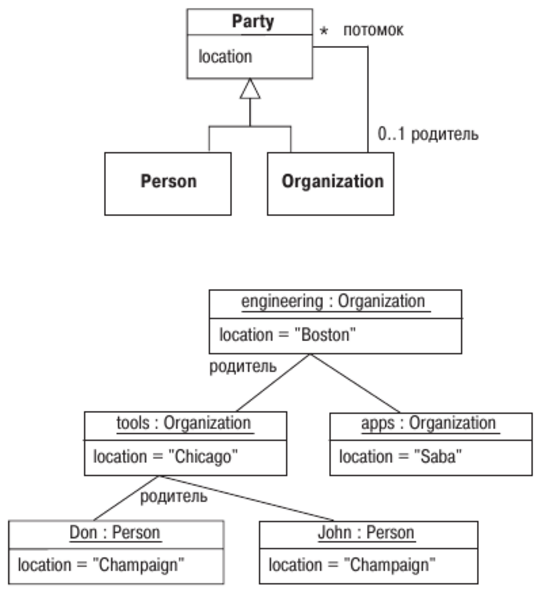
\includegraphics[width=\textwidth]{objectsDiagram.png}
				\end{center}
			\end{column}
		\end{columns}
	\end{frame}

	\begin{frame}
		\frametitle{Диаграммы компонентов}
		\begin{center}
			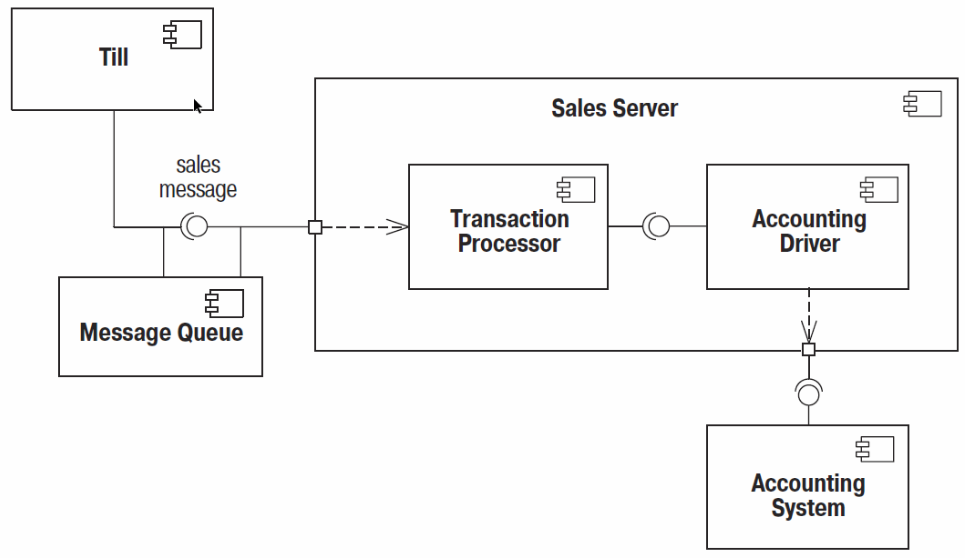
\includegraphics[width=0.9\textwidth]{componentDiagram.png}
		\end{center}
	\end{frame}

	\section{CASE-системы}

	\begin{frame}
		\frametitle{Computer-Aided Software Engineering}
		\begin{itemize}
			\item В 80-е годы термином CASE называли всё, что помогает разрабатывать ПО с помощью компьютера
			\begin{itemize}
				\item Даже текстовые редакторы
			\end{itemize}
			\item Теперь --- прежде всего средства для визуального моделирования (UML-диаграммы, ER-диаграммы и т.д.)
			\item Отличаются от графических редакторов тем, что ``понимают'', что в них рисуют
			\item Нынче чаще используются термины ``MDE tool'', ``UML tool'' и т.д.
		\end{itemize}
	\end{frame}

	\begin{frame}
		\frametitle{Типичная функциональность CASE-инструментов}
		\begin{itemize}
			\item Набор визуальных редакторов
			\item Репозиторий
			\item Набор генераторов
			\item Текстовый редактор
			\item Редактор форм
			\item Средства обратного проектирования (reverse engineering)
			\item Средства верификации и анализа моделей
			\item Средства эмуляции и отладки
			\item Средства обеспечения командной разработки
			\item API для интеграции с другими инструментами
			\item Библиотеки шаблонов и примеров
		\end{itemize}
	\end{frame}

	\begin{frame}
		\frametitle{Примеры CASE-инструментов}
		\begin{itemize}
			\item ``Рисовалки''
			\begin{itemize}
				\item Visio
				\item Dia
				\item SmartDraw
				\item Creately
			\end{itemize}
			\item Полноценные CASE-системы
			\begin{itemize}
				\item Enterprise Architect
				\item Rational Software Architect
				\item MagicDraw
				\item Visual Paradigm
				\item GenMyModel
			\end{itemize}
			\item Забавные штуки
			\begin{itemize}
				\item \url{https://www.websequencediagrams.com/}
				\item \url{http://yuml.me/}
				\item \url{http://plantuml.com/}
			\end{itemize}
		\end{itemize}
	\end{frame}

	\section{Паттерны проектирования}

	\begin{frame}
		\frametitle{Паттерны проектирования}
		\framesubtitle{Книжка}
		\begin{columns}
			\begin{column}{0.7\textwidth}
				\textbf{Приемы объектно-ориентированного проектирования. Паттерны проектирования}
				
				Э. Гамма, Р. Хелм, Р. Джонсон, Дж. Влиссидес

				Design Patterns: Elements of Reusable Object-Oriented Software
			\end{column}
			\begin{column}{0.3\textwidth}
				\begin{center}
					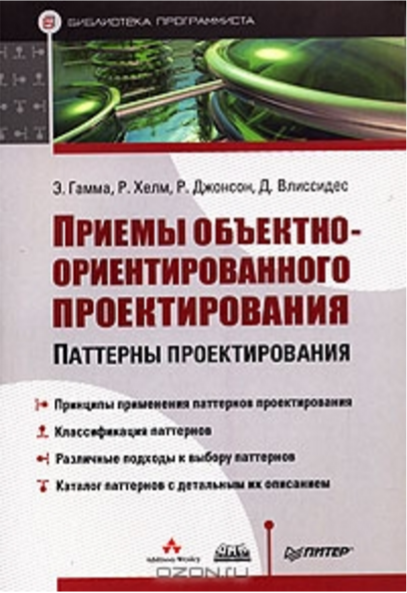
\includegraphics[width=0.9\textwidth]{patternsBookCover.png}
				\end{center}
			\end{column}
		\end{columns}
	\end{frame}

	\begin{frame}
		\frametitle{Паттерны проектирования}
		\textbf{Паттерн проектирования} --- повторимая архитектурная конструкция, являющаяся решением некоторой типичной технической проблемы
		\begin{itemize}
			\item Подходит для решения целого класса проблем
			\item Переиспользуемость знаний
			\item Унификация терминологии
			\item Простота в изучении
			\item Опасность карго-культа!
		\end{itemize}
		А ещё есть \textbf{антипаттерны} --- часто встречающиеся неправильные решения типичной проблемы
	\end{frame}

	\begin{frame}
		\frametitle{Пример паттерна, компоновщик (1)}
		\begin{center}
			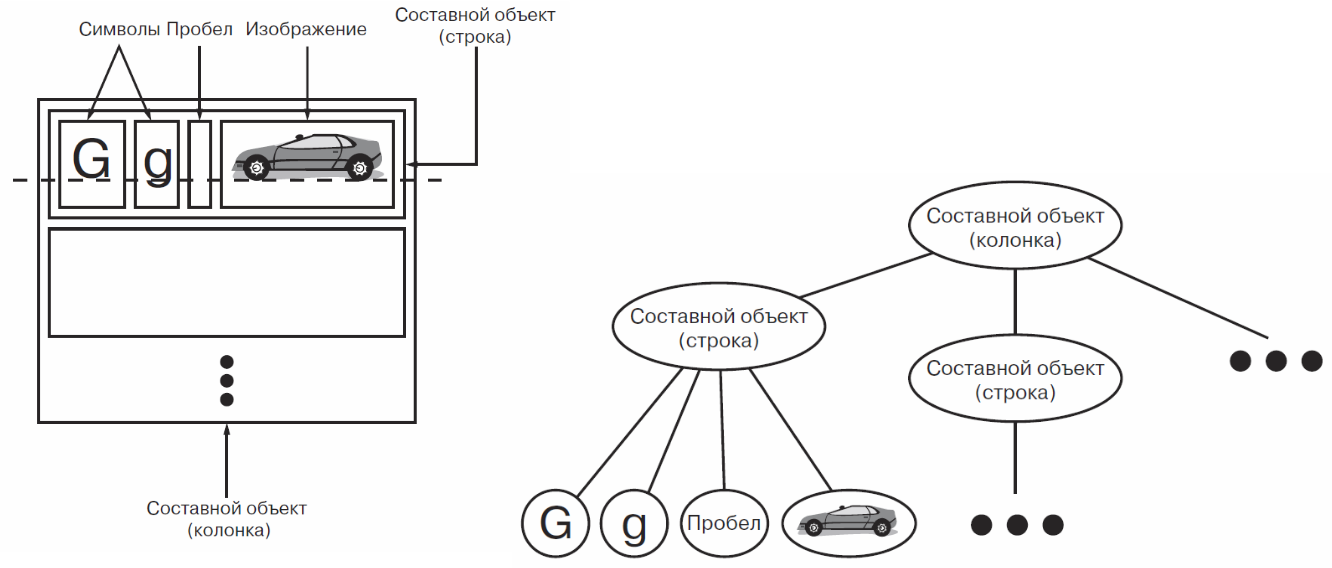
\includegraphics[width=0.9\textwidth]{documentComposition.png}
		\end{center}
	\end{frame}

	\begin{frame}
		\frametitle{Пример паттерна, компоновщик (2)}
		\begin{center}
			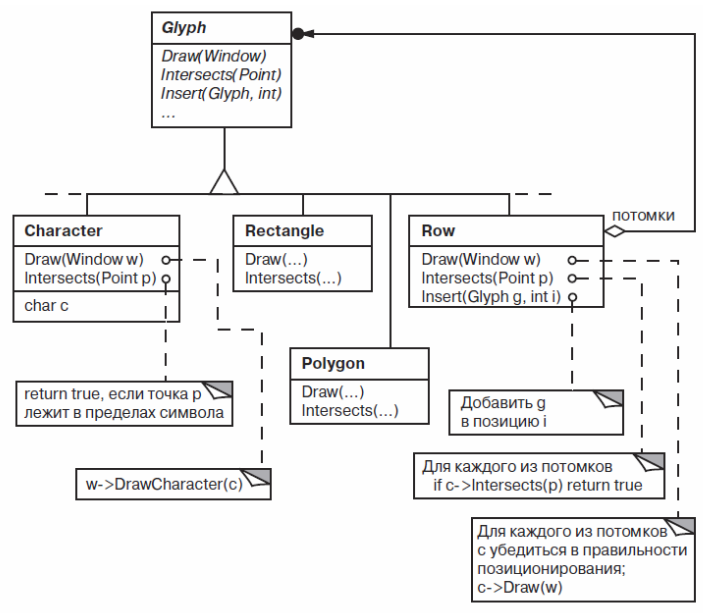
\includegraphics[width=0.65\textwidth]{glyphs.png}
		\end{center}
	\end{frame}

	\begin{frame}
		\frametitle{Пример паттерна, компоновщик (3)}
		\begin{center}
			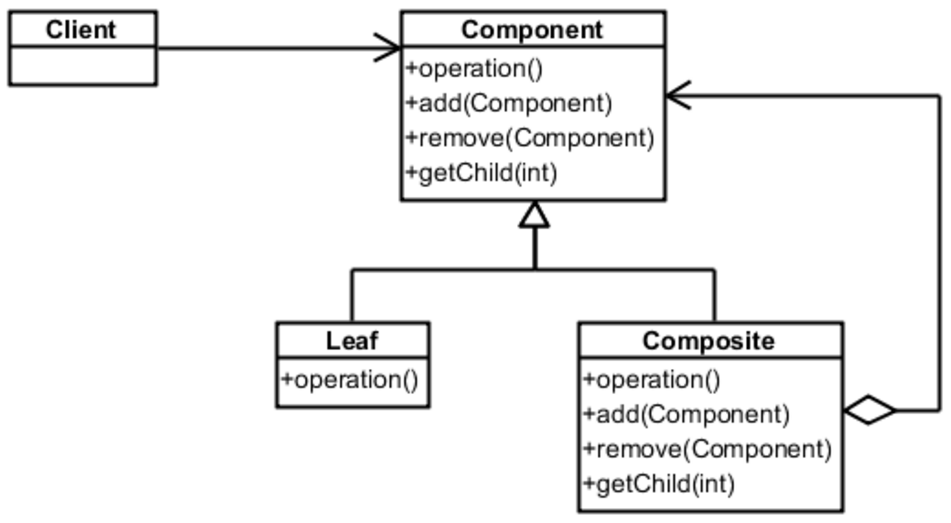
\includegraphics[width=0.7\textwidth]{composite.png}
		\end{center}
	\end{frame}

	\begin{frame}
		\frametitle{Ещё пример, паттерн ``Стратегия'' (1)}
		\begin{center}
			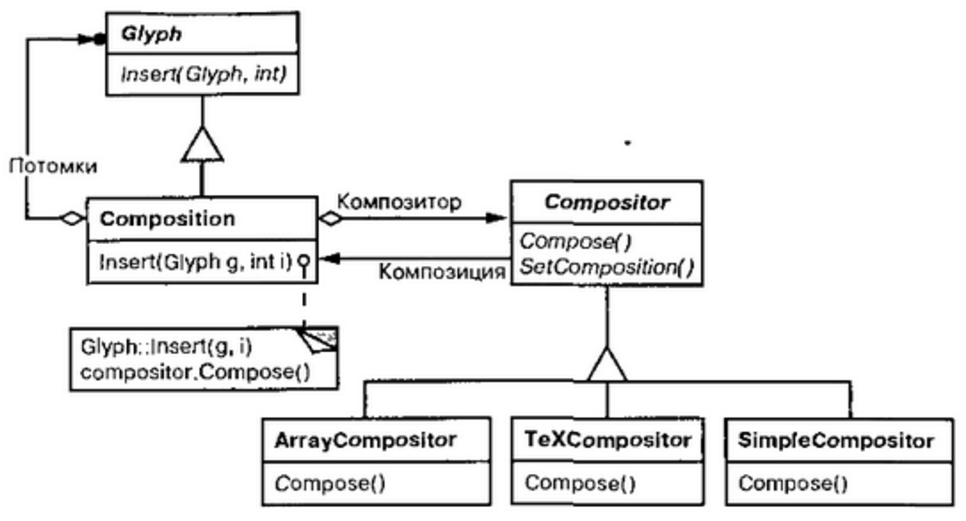
\includegraphics[width=0.9\textwidth]{glyphCompositor.png}
		\end{center}
	\end{frame}

	\begin{frame}
		\frametitle{Ещё пример, паттерн ``Стратегия'' (2)}
		\begin{center}
			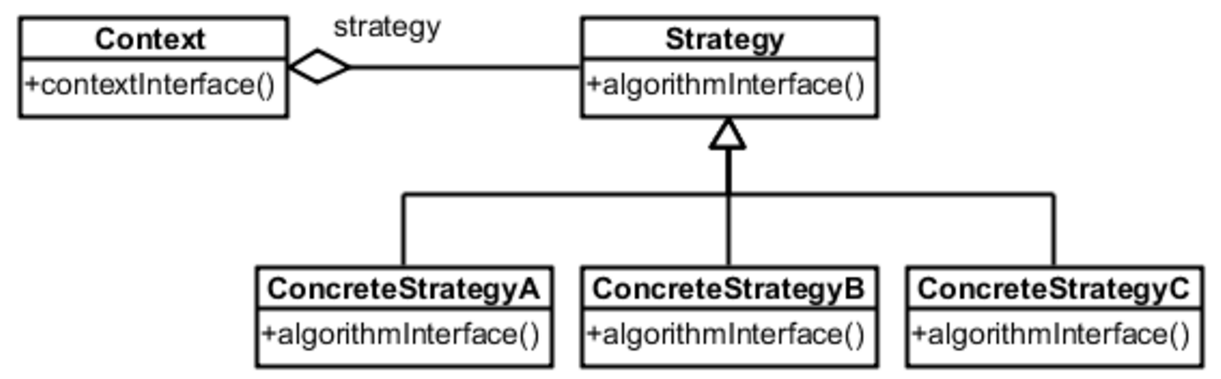
\includegraphics[width=0.9\textwidth]{strategy.png}
		\end{center}
	\end{frame}

\end{document}